\begin{frame}\frametitle{Presentación del curso}
  \textbf{Objetivos:}
  \begin{itemize}
  \item Aprender los conceptos básicos de visión computacional enfocados a la solución de un problema particular: dotar de autonomía a un robot móvil
  \item Implementar dichos conceptos en un ambiente simulado
  \item Familiarizar al estudiante con diversas herramientas de software como ROS, Numpy y OpenCV
  \end{itemize}
\end{frame}


\begin{frame}\frametitle{Contenido}
  \begin{itemize}
  \item Introduction
  \item Procesamiento de Imágenes
  \item Modelo de una cámara
  \item Espacios de color
  \item Características (\textit{Features})
  \item Clasificación y reconocimiento
  \item Redes Neuronales
  \item Navegación visual 
  \end{itemize}
  \[\]
  \textbf{Bibliografía recomendada:}
  \begin{itemize}
  \item \url{https://drive.google.com/drive/folders/1gb7VQJG5eUkCvCginRHHGn5lez6VASBJ?usp=sharing}
  \item \url{https://drive.google.com/drive/folders/1Epl2b51xEJzCvzfugBD1i7xGdKYdJucy?usp=sharing}
  \end{itemize}
\end{frame}

\begin{frame}\frametitle{Forma de trabajo}
  \begin{itemize}
  \item Horario: Viernes de 10:00 a 13:00.\\
  \item Para la realización de ciertas tareas se utilizará el simulador Gazebo junto con la plataforma ROS Noetic. Este software corre en el sistema operativo Ubuntu 20.04. Las prácticas implicarán escribir código para lo cual se utilizará el repositorio\\
    \url{https://github.com/mnegretev/ComputerVisionForRobotics-2023-2}\\
    Si no se desea instalar el sistema operativo de forma nativa, en el repositorio hay una máquina virtual con todo el software ya instalado.
  \item Para el uso del material del curso, se recomienda manejar las siguientes herramientas:
    \begin{itemize}
    \item Sistema operativo Ubuntu
    \item Lenguajes Python y C++
    \item Software de control de versiones Git
    \end{itemize}
    Un conocimiento a nivel introductorio es suficiente.
  \item Los códigos de cada práctica se subirán al repositorio en la rama asignada para cada estudiante.
  \item Los reportes escritos se entregarán al inicio de la clase en la fecha asignada.
  \end{itemize}
  Habrá un grupo en Google Classroom para todos los avisos. 
\end{frame}

\begin{frame}\frametitle{Forma de evaluar}
  Rubros a evaluar:
  \begin{table}
  \begin{tabular}{lr}
    Prácticas & 50\%\\
    Examen    & 50\%\\
  \end{tabular}
  \end{table}
\end{frame}


\section{Introducción}

\begin{frame}\frametitle{¿Qué es la visión computacional?}
  \begin{itemize}
  \item \textbf{Visión Humana: } Se puede concebir como una tarea de procesamiento de información, que obtiene significado a partir de los estímulos percibidos por los ojos.
  \item \textbf{Visión Computacional: } Desarrollo de programas de computadora que puedan \textit{interpretar} imágenes. Es decir, realizar la visión humana por medios computacionales. 
  \end{itemize}
  \begin{figure}
    \centering
    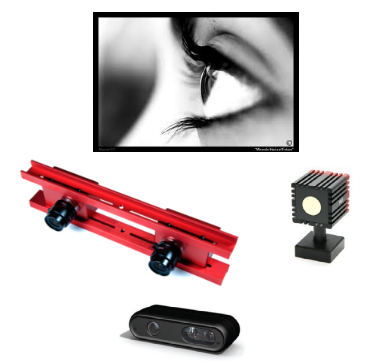
\includegraphics[width=0.5\textwidth]{Figures/VisionConcept.png}
  \end{figure}
\end{frame}

\begin{frame}\frametitle{Teoría de Marr}
“Visión es un proceso que produce, a partir de imágenes del mundo externo, una descripción que es útil para el observador y que está libre de información irrelevante.” (Marr, 1976).\\
El fenómeno de la visión lo podemos considerar como el producto de un sistema de procesamiento de información.\\

Marr propone los siguientes tres niveles de construcción de un sistema de procesamiento de información:\\
\begin{enumerate}
\item Teoría Computacional (¿Cuál es el problema por resolver?)
\item Representación y algoritmos (Estrategía usada para resolverlo)
\item Implementación (Realización física, software y hardware)
\end{enumerate}
Es decir, la visión computacional sería un proceso parecido a la visión humana, similar en los niveles computacionales y de algoritmos, pero implementado de forma diferente: en hardware de procesamiento con sensores de visión. 
\end{frame}

\begin{frame}\frametitle{Visión Computacional}
  Por lo tanto, la tarea de la Visión por computadora es la construcción de descriptores de la escena con base en características relevantes contenidas en una imagen:
  \begin{columns}
    \begin{column}{0.5\textwidth}
\begin{figure}
    \centering
    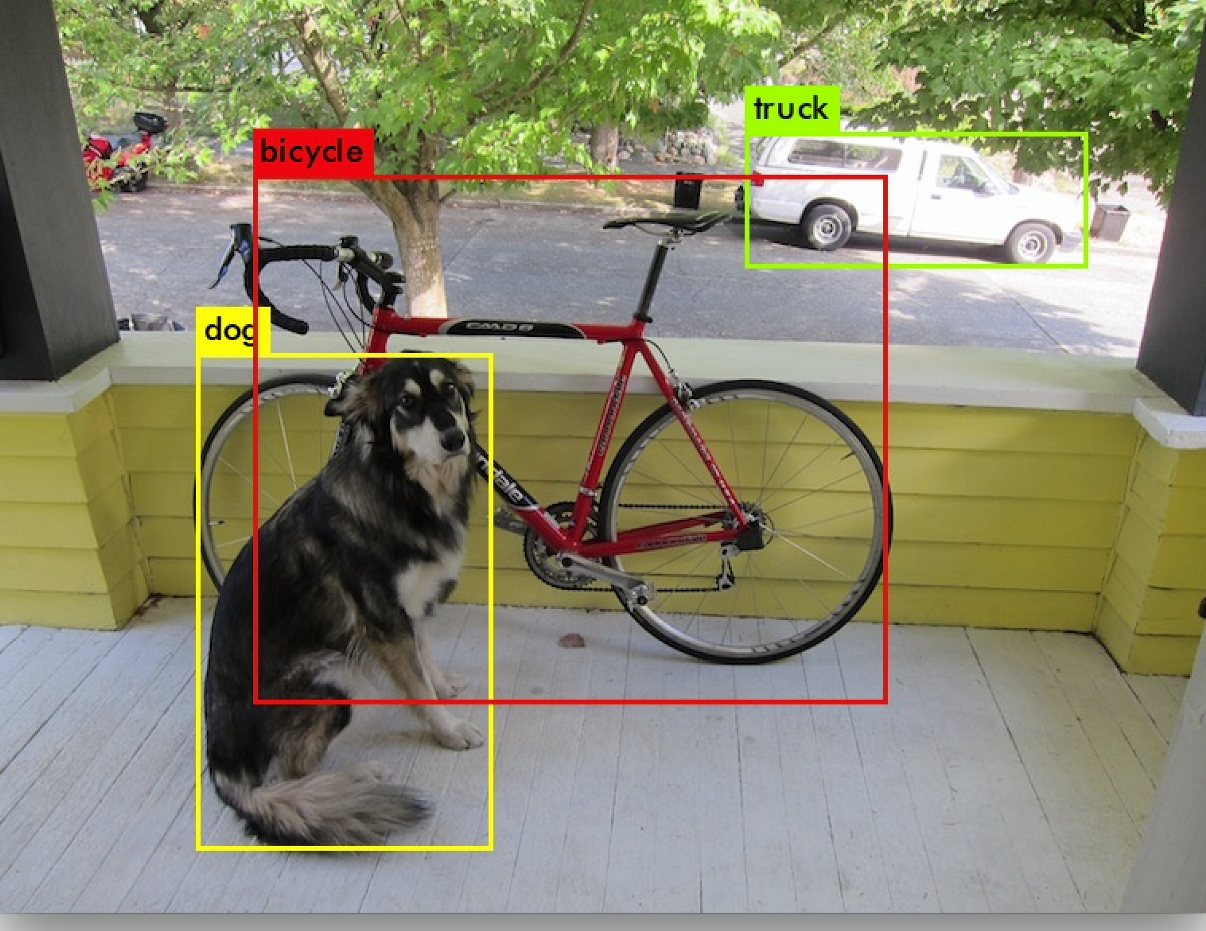
\includegraphics[width=0.8\textwidth]{Figures/Yolo.png}
\end{figure}
    \end{column}
    \begin{column}{0.5\textwidth}
\begin{itemize}
\item Objetos
\item Formas de Superficies
\item Colores
\item Texturas
\item Movimientos
\item Iluminación
\item Reflejos
\end{itemize}
    \end{column}
    \end{columns}
\end{frame}

\begin{frame}\frametitle{Vision Computacional vs Proc de Imágenes}
\begin{enumerate}
\item Procesamiento de imagenes: Es cualquier forma de procesamiento de señales donde la entrada es una imagen, la salida puede ser otra imagen o un conjunto de características o parámetros relacionados con la misma.
\item Visión Computacional: Estudio y aplicación de métodos que permiten a las computadoras “entender” el contenido de una imagen.
\item Visión Máquina: Es la aplicación de la visión por computadora en la industria y procesos de manufactura.
\end{enumerate}

\end{frame}

\begin{frame}\frametitle{Aplicaciones}
  Tareas que se pueden hacer con visión computacional (con aplicaciones a la robótica):
  \begin{itemize}
  \item OCR (Optical Character Recognition)
  \item Detección e identificación de rostros
  \item Reconocimiento de objetos
  \item Percepción para vehículos sin conductor
  \item Reconocimiento de gestos
  \end{itemize}
  Otras aplicaciones:
  \begin{itemize}
  \item Vigilancia
  \item Imagenología médica
  \item Consultas a bases de datos de imágenes.
  \item Percepción remota
  \end{itemize}
\end{frame}


\begin{frame}\frametitle{Esquema de Visión}
  \begin{figure}
    \centering
    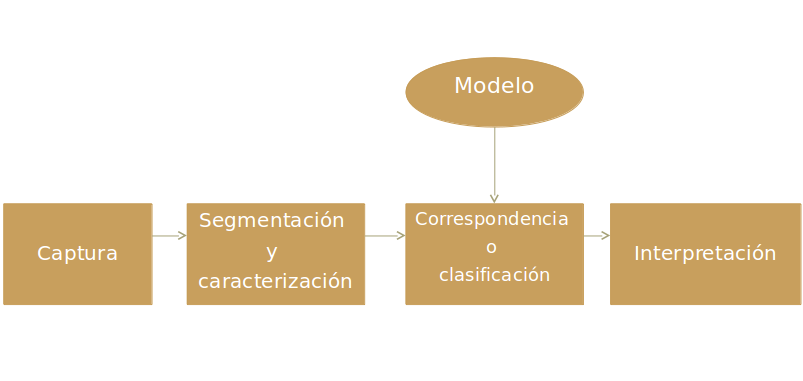
\includegraphics[width=1.0\textwidth]{Figures/VisionGeneralProcess.png}
  \end{figure}
\end{frame}


\begin{frame}\frametitle{Dificultades}

  El entorno real tiene una gran cantidad de variaciones en las imágenes de entrada.
  \begin{columns}
    \begin{column}{0.5\textwidth}
\begin{figure} %this figure will be at the right
    \centering
    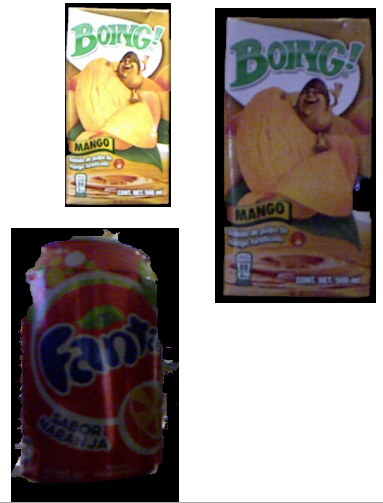
\includegraphics[width=0.5\textwidth]{Figures/VisionDificulties.png}
\end{figure}
    \end{column}
    \begin{column}{0.5\textwidth}
\begin{enumerate}
\item Iluminación
\item Orientación
\item Oclusión
\item Escala
\item Ruido
\item Desenfoque
\end{enumerate}
    \end{column}
  \end{columns}
\end{frame}

\begin{frame}\frametitle{Hardware y Software}
La computación con imágenes tiene mas de 30 años, sin embargo, en los últimos años, se ha incrementado considerablemente su desarrollo debido a:
\begin{enumerate}
\item Decremento en los precios 
\item Memoria con gran capacidad
\item Procesadores de propósito general de alta velocidad.
\item Existen scanners o camaras digitales que pueden ser utilizados para procesar imágenes propias.
\item Existen bibliotecas de software que contienen subrutinas de procesamiento de imágenes (opencv).
\end{enumerate}
\end{frame}


